\documentclass{standalone}
\makeatletter\AtBeginDocument{\@buildstepset{1,2,3}}\makeatother\usepackage{hsbcommon}
\begin{document}
\pgfplotsset{compat=1.18}
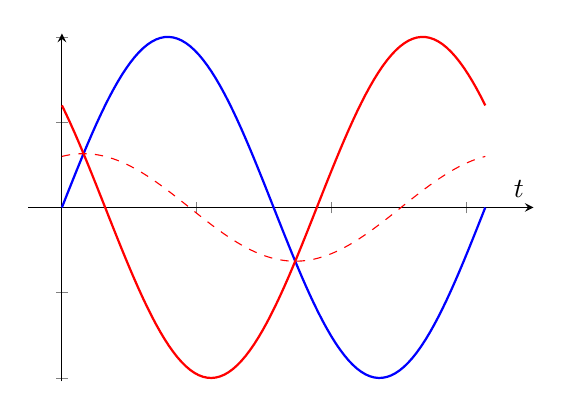
\begin{tikzpicture}
        % \draw[->] (0,0) -- (8,0) node[draw=none,right]  {$A$};
        % \draw[->] (0,-4) -- (0,4) node[draw=none,above]  {$B$};

        
    \begin{axis}[
        axis lines = middle,
        xlabel = $t$,
        ylabel = {},
        ymin=-102, ymax=102,
        xmin=-0.5, xmax=7,
        domain=0:2*pi,
        samples=100,
        width=8cm,
        height=6cm,
        yticklabel=\empty,
        xticklabel=\empty
    ]
    \ifstep{1}{
    \addplot [blue, thick] {sin(deg(x))*100} ;}
    \ifstep{2}{
    \addplot [red, thick] {sin(deg(x+2.5))*100};
    \addplot [red, dashed] {((sin(deg(x+2.5))*100)+(sin(deg(x))*100))/2};
    }
    \end{axis}
        

\end{tikzpicture}
\end{document}
